\chapter{研究设置}
\label{chp:data_description}

仿冒应用的生态是移动黑灰色产业研究中尚未被探明的一环。
为了补上这一研究空白,本文先提出了一系列针对仿冒应用的研究问题,再使用实证研究技术对这些问题一一解答。
实证研究需要数据支撑,在缺乏前人研究提供数据或分析的基础上,本研究从工业界直接获取真实世界的样本以完成调研。
本章介绍本研究的整体设置:先提出本文的研究问题,再介绍研究对象的选取(即从什么对象中获取研究数据),最后描述数据搜集思路方法与所得数据集和其他已有数据集的对比。


% \subsection{Workflow of Our Study}
\section{研究问题}

一方面,探明仿冒应用生态的重要一步是了解其本身特征,以协助后续研究中对仿冒应用的自动化辨识和指导一般消费者鉴别仿冒应用。
从直觉上看,仿冒应用与某一正版应用越相似,则越可能误导用户下载应用,使仿冒开发者获利。
在这一方面,为了解、验证仿冒应用特征,本文从相似度、影响应用被仿冒程度的因素及仿冒应用行为三点出发,提出了以下问题:
RQ1:仿冒应用和与之相对的正版应用的相似程度如何?
RQ2:是否存在显著影响应用被仿冒的严重程度的单一因素?
RQ3:仿冒应用作者制作出了怎样的仿冒应用?是否依然能提供原版应用的功能?

另一方面,仿冒应用的发布行为特征与仿冒应用本身特征同样重要,了解仿冒应用作者的发布特征有利于使市场方强化筛选、审查方案,防止仿冒应用流入市场。
由于应用开发者与应用证书的一对多关系(详见第二章),本研究借助仿冒应用的证书信息探究仿冒应用作者的行为。
在这一方面,为了解仿冒应用开发者行为特征,本文提出了以下研究问题:
RQ4:仿冒应用与开发者的对应关系如何?
RQ5:仿冒应用证书可以活跃多长时间?
RQ6:仿冒应用的上架行为是否有特征?

再进一步,应用市场中的用户反馈影响应用在市场上的分类排名,因此仿冒应用作者也可能操纵评论以增加自身应用的曝光率。
对应地,本研究提出研究问题如下:
RQ7:仿冒应用作者是否进行了排名欺诈行为?如果是,能否总结出类似行为的特点?

上述研究问题从三个不同角度,即仿冒应用基本特征、仿冒应用开发者发布行为的特征和仿冒应用的市场反馈对其进行探究。
这些问题的答案不仅可为后续研究提供仿冒应用的基础认知与检测思路,还能同时为普通消费者和应用市场在鉴别仿冒应用方面提供一定线索。
% \begin{figure}[htbp]
% 	\centering
% 	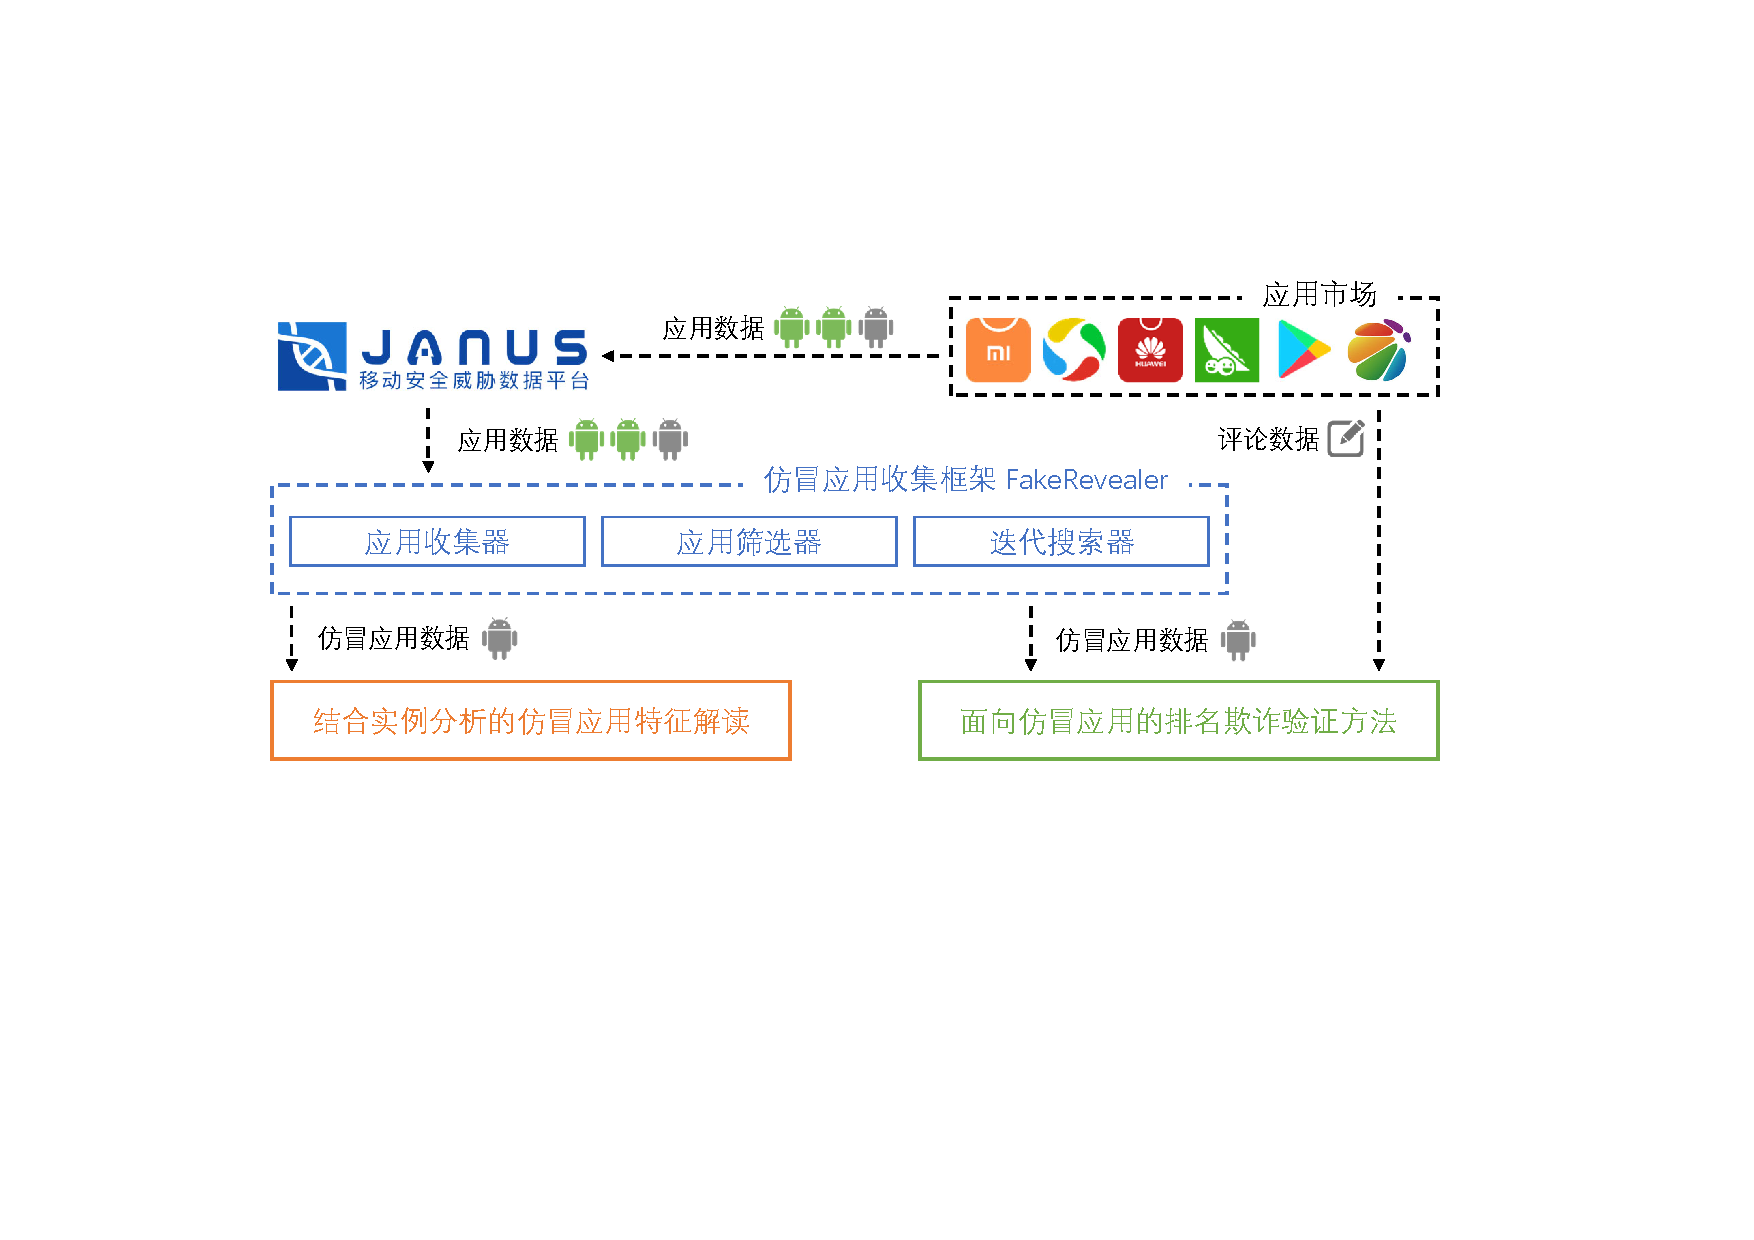
\includegraphics[width=\textwidth]{./Figures/edwin-overview}
% 	\caption{本文研究流程}
% 	\label{fig:Workflow}
% 	\vspace{-3mm}
% \end{figure}

% Fig.~\ref{fig:Workflow} shows the workflow of our study, which can be divided into two main phases:
% \autoref{fig:Workflow} 展示了本次实证研究的流程,其可以分为四个主要阶段:

% 1)\ \emph{数据收集} \quad
% 数据收集主要分为两个部分:正版应用信息的收集和仿冒应用的收集。
% 在正版应用信息收集的部分,本文选择了50个最热门的App作为目标应用,然后手动收集了跟这些App有关的信息;
% 仿冒应用信息收集方面,作者得到了上海犇众信息技术有限公司的帮助,得以接触从各个应用商店获得的大量的应用样本。
% 借助自动化分析框架\mytool,作者获得了大量仿冒应用的数据。

% 2)\ \emph{大规模数据挖掘} \quad
% 在这一步,我们对搜集到的仿冒样本数据进行分析,从三个视角完成了一次大规模数据挖掘。
% 三个视角分别是仿冒的基本应用特征、影响仿冒应用数量的因素和仿冒应用的发展轨迹,由浅入深,帮助读者理解仿冒应用的生态。

% 3)\ \emph{仿冒案例分析} \quad
% 之后,我们从收集的数据中选择了3个案例进行更深入的分析。
% 这三个案例在支持数据挖掘中的发现之外,揭示了更多仿冒应用开发者的行为特征。

% 4)\ \emph{市场反馈分析} \quad
% 在这个部分,我们从第三方应用市场中随机选取一部分应用,提取了用户对它们的所有历史评价,然后筛选出其中对仿冒应用的评价并分析,以期了解用户对这些应用持有的态度。
% 此基础上,我们还检测了仿冒应用与排名欺诈行为的关系,揭示移动黑灰产不同环节之间的关联。

\section{研究对象}
仿冒应用是一个跟正版应用相对的概念,所以需要先定义正版应用,再对仿冒应用进行探究。
因此,本研究先选取了一部分正版应用作为目标应用,再根据正版应用的信息搜寻仿冒应用,对搜集到的样本进行研究。

文献~\cite{kitchenham2002preliminary}指出,实证研究需要确保数据的准确性与全面性。
若在市场直接中随机挑选应用,将难以解释搜集到的应用是正版或是仿冒应用,进而不能保证数据的准确性,随机选取法并不适用于正版应用的选取。
因此,本研究参考了数据平台易观千帆的月度App排行榜\footnote{\url{https://qianfan.analysys.cn/refine/view/rankApp/rankApp.html}}。
该排行榜对超过1200个主流应用中的用户分享数据进行分析,汇总成应用热度(月度活跃用户数),按热度对应用进行排行。
一方面,该排行榜的数据来源是各应用``应用体验计划''中搜集所得的数据,数据本身具有一定真实性,可满足文献的准确性要求;
另一方面,排行榜中的应用均为主流应用,由知名度较高的开发者(如腾讯、百度、阿里巴巴等)开发,可认为排行榜上的应用均为正版应用,免去需要对搜集到的目标应用进行甄别的步骤;
此外,排行榜中的应用涵盖了多个领域,包括社交网络、资讯、移动购物、视频等,能满足数据收集中的全面性要求。
综上,从易观千帆平台选择目标应用是较为合适的方式。

\begin{table}[htbp]
	\renewcommand{\arraystretch}{1}
	\small
	\centering
	\caption{目标应用类别与各分类下应用}
	\vspace{1mm}
	\begin{tabular}{l c}
		\toprule
		{\bf 应用类别}                            & {\bf 应用名}                                               \\
		\midrule
		{社交网络}                                & {微信、QQ、新浪微博}                                       \\
		\rowcolor{gray!15}视频                    & {爱奇艺、腾讯视频、优酷、快手、抖音、火山小视频、西瓜视频} \\
		{生活}                                    & {支付宝、高德地图、百度地图、美团、墨迹天气、滴滴出行}     \\
		\rowcolor{gray!15}移动购物                & {淘宝、京东、拼多多}                                       \\
		\multirow{2}*{系统工具}                   & {WiFi万能钥匙、搜狗输入法、腾讯手机管家、360手机卫士、}    \\
		~                                         & {猎豹清理大师、360清理大师、WiFi管家、讯飞输入法}          \\
		\rowcolor{gray!15}                        & {百度、腾讯新闻、QQ浏览器、今日头条、}                     \\
		\rowcolor{gray!15} \multirow{-2}{*}{资讯} & {UC浏览器、网易新闻}                                       \\
		\multirow{2}*{应用市场}                   & {应用宝、华为应用市场、OPPO应用市场、}                     \\
		~                                         & {360手机助手、百度手机助手、小米应用市场}                  \\
		\rowcolor{gray!15}{音乐}                  & {酷狗音乐、QQ音乐、酷我音乐盒、全民K歌、网易云音乐}        \\
		{游戏}                                    & {王者荣耀、开心消消乐}                                     \\
		\rowcolor{gray!15}{摄影录像}              & {美图秀秀、美颜相机}                                       \\
		{商务办公}                                & {WPS Office、QQ邮箱}                                       \\
		\bottomrule
	\end{tabular}
	\label{table:taget_app}
\end{table}

该平台月度App排行榜的排名前50的热门应用被挑选作为本文的目标应用。
从功能角度入手,50个App被归入11个类别,分别为社交网络、视频、生活、移动购物等,详情可见\autoref{table:taget_app}。
作者手动从这50款App的官方网站上下载了这批应用的最新版本,作为正版应用的参考版本,寻找与之相关的仿冒应用进行后续研究。


\section{数据收集}
鉴于目前学术界中与仿冒应用直接相关的数据集较为稀缺,从工业界中系统地收集所需的仿冒应用数据来完成本次调研是最为直观合适的方法。
本节先根据上述的研究问题划定本研究所需的研究数据类型,再介绍如何对数据进行收集。

% \noindent {\bf Collected Dataset.}
\subsection{数据类型与收集方式}

综合研究问题,本研究需获取的数据类型可分为以下三部分:一、分析仿冒应用特征所需的应用基本信息;二、分析应用发布特征所需的应用证书信息、上架时间等元数据;三、分析仿冒应用是否进行排名欺诈行为的评论数据。

确定目标应用后,可在市场中寻找与目标应用相似的应用,提取其数据整理成集,满足一、二部分的数据需求。
但要获取足量的仿冒应用数据以组成数据集是一个较有挑战性的任务,有难点如下:
\begin{itemize}
	\item 研究者要从多个不同的应用市场中爬取App样本,每个应用市场都有不同的网页编码,甚至有反爬虫策略,不存在一个爬虫脚本对所有应用市场数据都通用的场景;
	\item 各个应用市场架上的App数量庞大,研究者需要有效地筛选出与目标应用有关的样本;
	\item 对于收集到的大量数据,研究者需要一个轻量级的解决方案快速判断获得的App样本为正版应用或是仿冒应用。
\end{itemize}

为应对第一个挑战,作者与工业界合作,利用犇众信息公司的Janus平台对各大应用商店进行样本爬取,获取应用样本信息。
该平台自2017年起就开始对各大应用商店的App进行样本收集,可向用户提供各项App信息。
如\autoref{fig:Janus-data}显示,Janus平台至今已收集到上千万个App样本,可满足本研究数据采集需求。
除样本信息外,Janus也提供按规则搜索功能,用户可创建规则过滤平台中的应用数据,以获取所需应用App样本。
因此,视Janus平台为从各大应用市场中收集应用样本的代理,借助Janus平台获取各市场中的应用信息。

\begin{figure}[htbp]
	\centering
	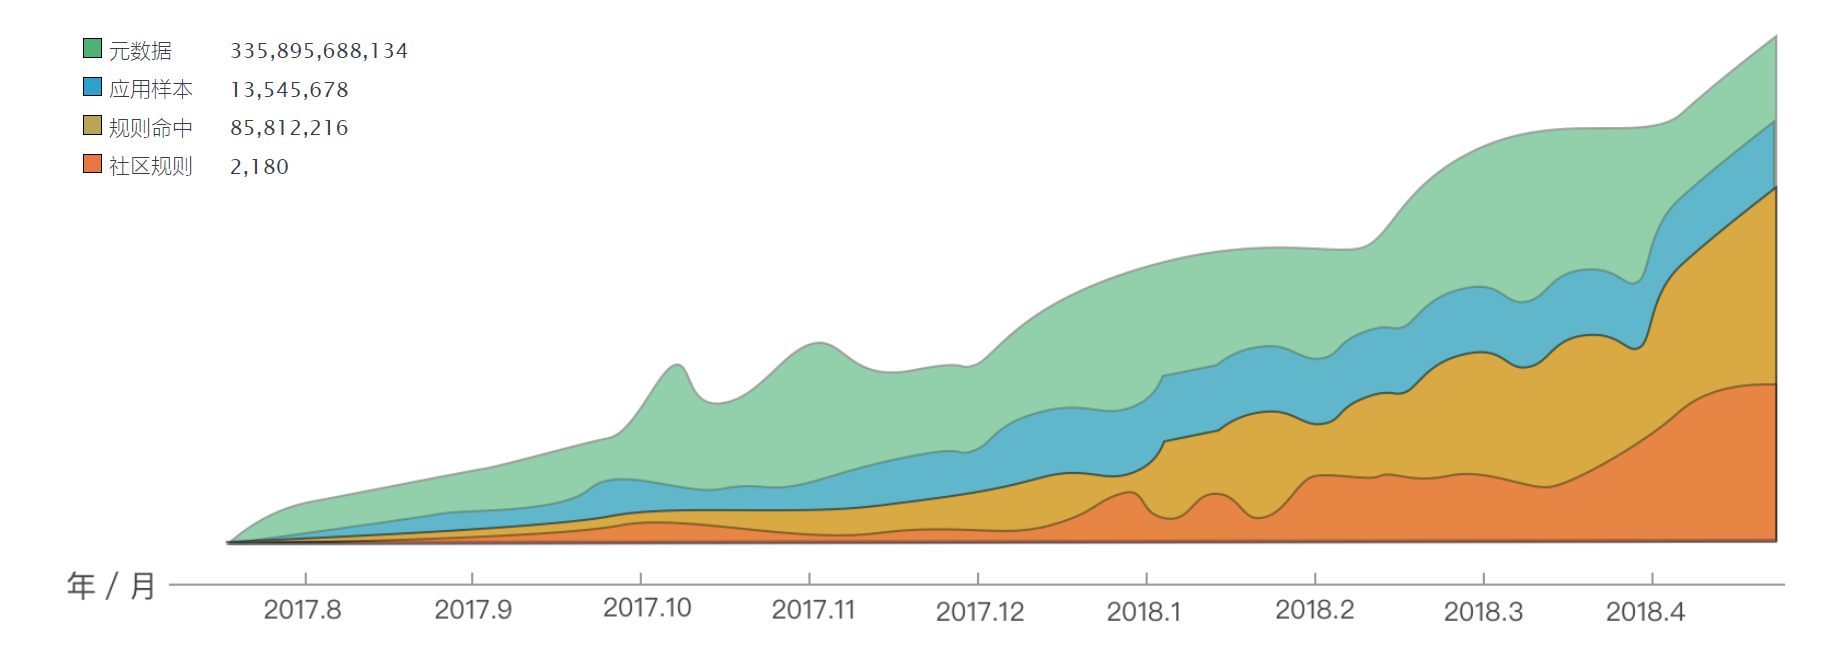
\includegraphics[width=\textwidth]{./Figures/edwin-Janus-data.png}
	\caption{Janus平台上的数据规模时序图}
	\label{fig:Janus-data}
	\vspace{-5mm}
\end{figure}


为应对第二个挑战,本研究提出了基于广度优先搜索(Breadth-First Search,简称BFS)算法的搜索框架\mytool,迭代收集与目标应用相关的样本,整体流程可见\autoref{fig:FakeRevealer}。
具体地,对于每一款目标应用,\mytool 的收集流程分为三个部分:先以正版应用样本的\emph{包名}和\emph{应用名}作为查询条件放入迭代搜索器,迭代搜索器发出查询请求,从Janus平台中收集与目标应用相关的所有App样本,提取出样本的相关数据返回至应用收集器;
其后,应用收集器将数据转移至应用过滤器,利用过滤器判断收集到的应用数据源于正版应用或仿冒应用,保存仿冒应用数据,提取出正版应用的\emph{包名}和\emph{应用名};
最后,将上一步中获得的新的正版应用信息(\emph{包名}和\emph{应用名})再次放入迭代搜索器,开始下一次循环,从Janus中进行查询,获取更多与正版应用相关的样本。

\begin{figure}[htbp]
	\centering
	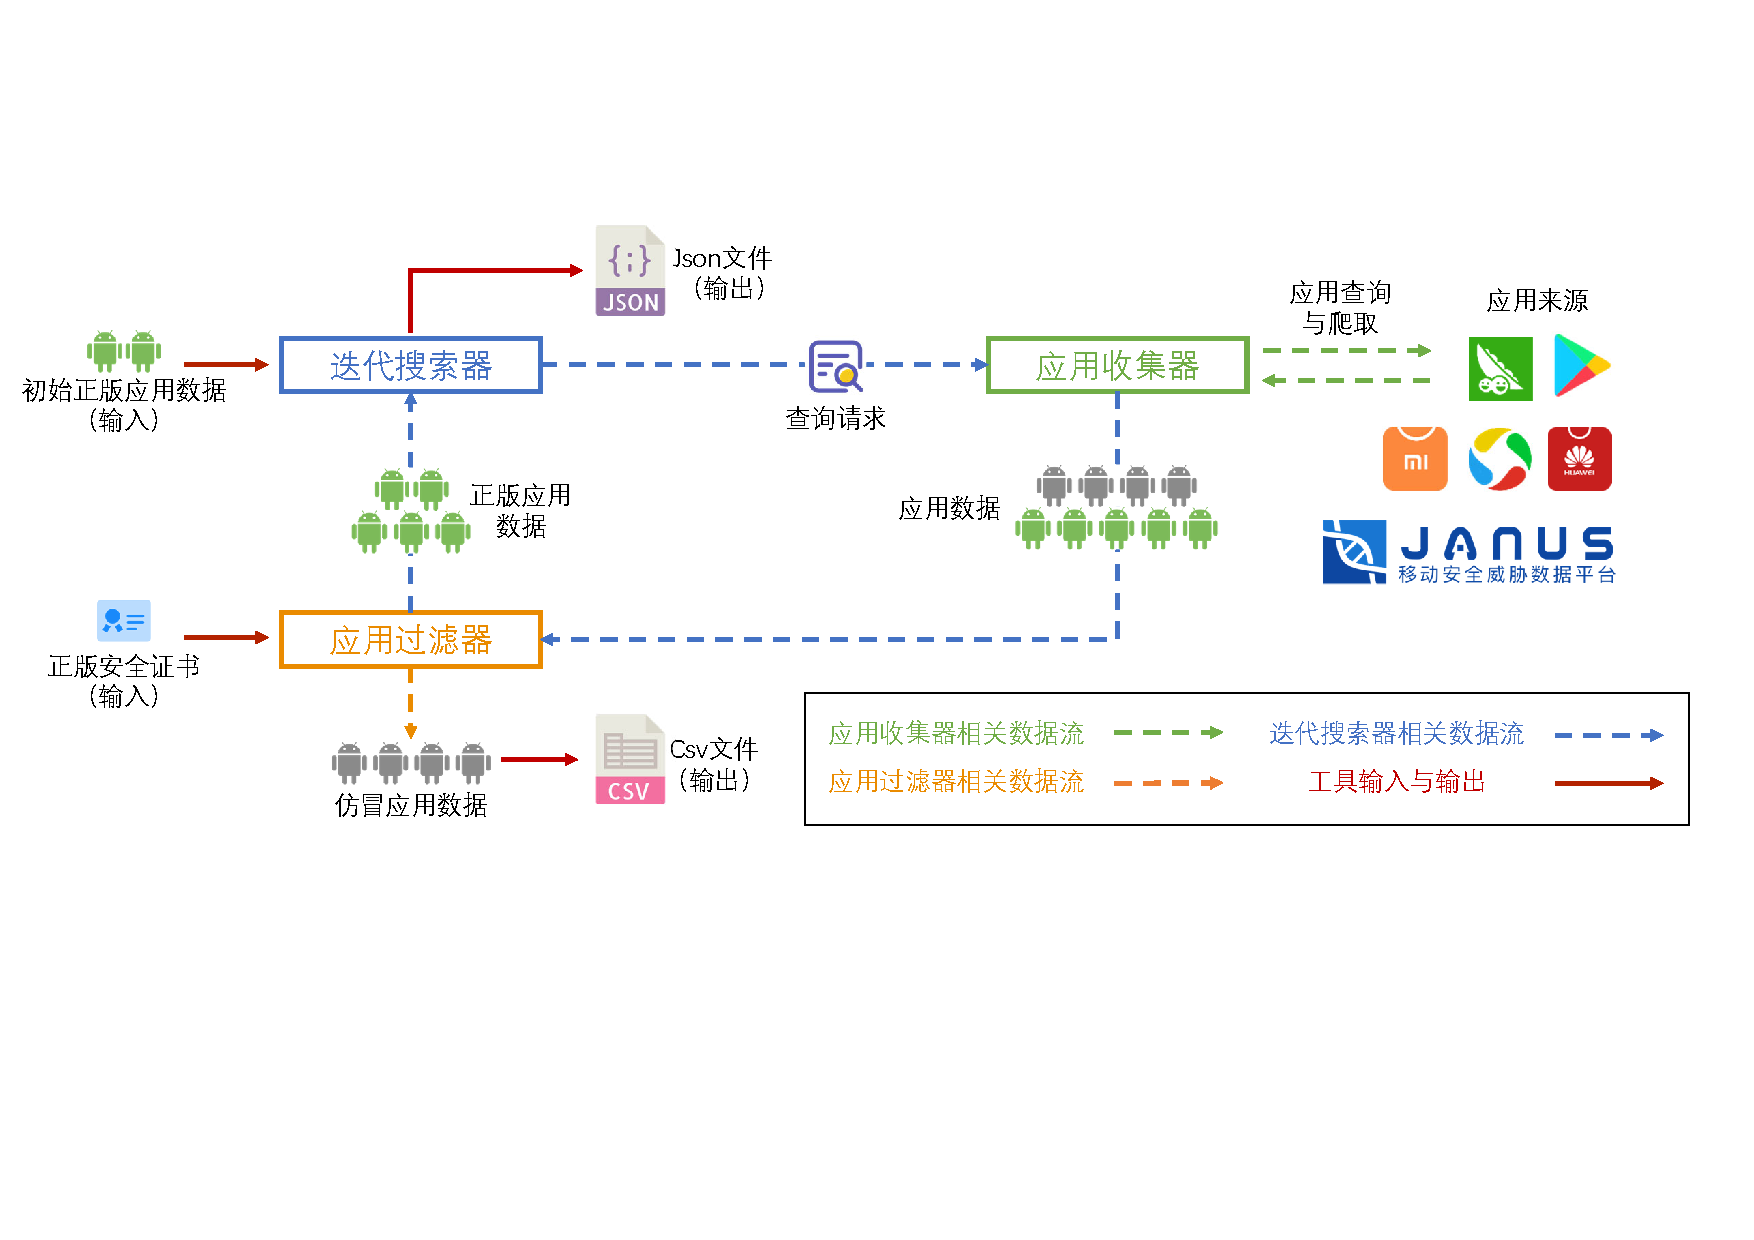
\includegraphics[width=\textwidth]{./Figures/edwin-fakerevealer}
	\caption{\mytool 整体流程}
	\label{fig:FakeRevealer}
	\vspace{-3mm}
\end{figure}

第三个挑战,可利用Android签名证书机制(详见第二章)解决。
对某个APK安装包而言,该机制提供了其被最后一次修改时的修改人信息。
因此,对于任一个被\mytool 收集到的APK,均可归入以下三种情况:

第一,该APK为正版应用,由正版开发者开发,也并未被篡改,应用证书与正版应用证书一致,是目标应用的某一版本;
第二,该APK原本为正版应用,由正版开发者开发,但被仿冒应用开发者解包篡改,加入、删除或修改了部分数据,成为仿冒应用。
然而,根据Android的打包流程与签名证书机制,仿冒应用开发者无法通过原版证书为该APK重新打包,因此该APK的应用证书被替换为仿冒应用开发者的证书;
第三,该APK由仿冒应用开发者开发,由于仿冒应用开发者不具有正版开发者的私钥,不能为该APK签署正版应用证书,因此该APK具有仿冒应用开发者的证书。

综上,对于收集到的某一应用信息,若其证书信息可与目标应用的应用证书信息相对应,则可认为该应用为正版应用;
相反,只要其应用证书信息与正版应用信息不符,无论其为被篡改的原正版应用,或是仿冒应用开发者从新开发的仿冒应用,均可划入仿冒应用范畴。

本研究从360手机助手应用市场中随机挑选了856个应用,爬取这批应用的所有评论作为第三部分数据。
国内应用商店市场监测报告~\cite{ChineseAppStoreReport}显示,360手机助手应用市场为国内占有市场份额最大的应用市场,以360手机助手为收集对象,可使数据具有一定代表性。
另外,与小米应用市场、OPPO应用市场等手机厂商推出的应用市场不同,360手机助手并非预置于手机系统中,因此可认为该应用市场用户喜好不与任一厂商的手机用户喜好强相关,在用户分布上具有更好的全面性。
对随机应用进行评论采集,而非针对特定应用进行评论采集也是出于相同考虑。
由于该856个应用为随机挑选所得,本研究认为这批数据具有一定的代表性,可反映整个市场的评论分布情况。

\subsection{数据概览}
\label{sec:data_overview}

如上节所述,本研究收集到的内容可分为两类:应用数据与评论数据。

应用数据方面,从易观千帆提供的数据榜单中,本研究选择了分属11个不同的应用类别的50个最热门的App作为目标应用,。
由于App的应用名可能会在App更新迭代的时候随之变更,作者用近似BFS的策略,从50种App中一共记录了198个不同的应用名以挖掘仿冒样本。

在这50款App中,以下三款App的样本并不能在市面上找到:\emph{OPPO 应用商店},\emph{华为应用商店}和\emph{小米应用商店}。
因为这三款App都是由手机设备厂商开发和预装在对应品牌的手机中的,仅供这些品牌的用户使用,并不在其他应用市场上提供下载。
当然,这也是这三款App热度高的原因——这几款App都被预装到了对应手机品牌厂商的每一部Android设备中,而OPPO、华为和小米又是国内最大的几家手机厂商,这几款App自然也会有庞大的用户基数。
因此,本研究最后的目标应用只有47款。

对这47款目标应用,\mytool 共检索到138,106个应用样本,样本源于29个不同渠道。
其中,69,614个应用样本持有官方开发者证书,52,638个应用样本并不具有官方证书。
余下部分应用样本为某些应用的发布在不同应用市场同一版本,在对各样本计算SHA1码去重筛选后被排除(共计15,854个)。
样本SHA1码是使用SHA1哈希算法对整个APK文件进行数据摘要之后获取到的编码串,可认为每个样本都有独一无二的SHA1码。

评论数据方面,本次研究一共爬取到了267,397名用户的365,461条评论,其中6款仿冒应用的所有历史评论共计3,591条,来自2,946名用户,每条评论数据由5项信息组成,除\emph{评论内容}、\emph{评价等级}和\emph{来源应用}三项必要信息外,还包括\emph{评论用户}与\emph{评论时间}以保留评论间的潜在联系。
在本研究收集评论的所有856个应用中,有6款应用与先前仿冒应用数据中的包名对应。
本研究的仿冒应用列表为针对50个热度最高的目标应用整理而成,而收集评论的应用在整个市场范围内随机挑选,此处仿冒应用占总体应用比例较小,不意味整个市场中的仿冒应用数量偏少。


\subsection{相关数据集}

作为软件工程方向的研究热点,Android应用研究一直广受关注。
在Android应用数据集方面,为推进Android恶意应用研究,一些安全厂商整理出了恶意应用数据集,使研究者免于数据收集之苦;部分论文中亦有公开的Android应用集可供参考。
较为著名的数据集有Android Malware Genome Project(Genome数据集),Drebin数据集,AMD数据集和AndroZoo数据集。

Genome数据集~\cite{Zhou2012DissectingAM}中的样本由Yajin Zhou等人持续收集一年余所得,其中包含了超过1,200个Android恶意应用,涵盖了收集时市面上存有的大部分恶意应用家族。
经过对数据集中恶意样本的详尽分析,Yajin Zhou等人总结了重打包、更新攻击和路过式下载(Drive-by Download)三种恶意应用的安装途径,并揭示了特权提升,远程控制,恶意扣费和信息收集四种恶意行为的方式,该数据集在后人研究中多被用于训练自动化恶意应用分类器。
该数据集收集的时间为2010年8月至2011年10月间,但已不再被维护。
Android系统在其后不断更新迭代,故其中的样本已有部分因兼容性问题不能再被安装到具有较新版本Android系统的设备上。
与该数据集类似的还有与2010年8月至2012年10月间收集的Drebin数据集~\cite{arp2014drebin},该数据集为Genome的超集,共包含涵盖了源于179个不同恶意应用家族的5,560个恶意样本。
AMD数据集~\cite{li2017android}则包含了从2010年至2016年间收集的24,553个样本,样本被分类至71个恶意应用家族的135个变种中,与Genome数据集和Drebin数据集相比,提供了更接近现状的恶意应用数据画像。
除去时间导致的兼容性问题,虽然Genome、Drebin和AMD三个数据集中的样本覆盖较为全面,但其收集对象已明确为产生恶意行为的``恶意应用'',而本文研究对象为模仿热门应用的仿冒应用,两者有所区别,因此直接使用三个数据集中的样本进行分析并不合适。

AndroZoo是一个仍在不断收集应用的数据集~\cite{li2017androzoo++}。
该数据集从包括Google Play应用商店、小米应用商店、安智网等多个数据源进行数据收集,现已包含超过一千两百万个应用样本。
一方面,AndroZoo的数据比前述数据集更新,更能反映应用市场现状;另一方面,比起Genome、Drebin和AMD三个针对恶意应用进行收集的数据集,AndroZoo收集的对象不限于恶意应用。
该应用集利用VirusTotal对所得的应用进行扫描,标记出被报告为恶意应用的样本;同时,维护者也整理了数据集中的重打包应用信息,为学者提供翔实的重打包应用相关的样本数据:该数据集的重打包应用目录共提供了2,776个原版应用样本对应的15,297个重打包样本。
与只针对恶意应用进行收集的数据集相比,同时收录重打包应用数据的AndroZoo数据集可用于更广泛的Android应用研究。
然而,重打包应用只是仿冒应用的其中一种形式,仿冒应用还包括仿照正版应用外观制作的应用程序,该数据集的重打包应用列表未能满足本文研究的数据需求。
因此,在对上述四个数据集进行调研对比后,作者选择重新构建仿冒应用数据集,以完成本文研究。

在评论数据集方面,已知数据集众多,大多源于大型网站。
大众点评于2011年11月至2013年11月期间收集了近万条评论~\cite{li2017bimodal};美国点评网站Yelp、TripAdvisor和电商网站Amazon各有其收集的真实数据,Yelp数据集包括了美国多家城市的数十万条餐厅点评~\cite{rayana2015collective, shehnepoor2017netspam},TripAdvisor数据集包括3万条评论~\cite{wu2010distortion},Amazon数据集中具有583万条评论,涵盖书籍、音乐、DVD/VHS等多个领域~\cite{jindal2008opinion};源于知名电影网站IMDB的评论数据集包含5万条影评~\cite{maas2011learning}。
少数数据集由学者在研究中公开,如Ott公布了其在相关研究中使用的数据集~\cite{ott2011finding},相关数据由两部分组成,真实数据部分从TripAdvisor中采集所得,虚假评论部分在Amazon的众包平台获取。
具体地,研究者在众包平台上以1美元为酬劳,请求用户对芝加哥的20家受欢迎酒店构想积极评论,以组成虚假评论数据集,最终得到了真实数据、虚假评论各400条的数据集。
Li在后续研究~\cite{li2014towards}中扩充了该数据集,让其涵盖了酒店、餐厅和医院三个领域,并加入了来自领域专家的虚假评论。

已有评论数据集面向的领域众多,但本文前期调研显示,尚未有针对应用市场评论的数据集公开可用。
本研究收集应用市场的评论数据的目的是勘查仿冒应用是否具有排名欺诈行为,来自其他领域的评论数据集并不符合收集需求。
因此,本研究仍需自行采集数据。
以上评论数据集仍对本文评论数据收集有所启发:大型网站中可更易于获取有效数据,因此本研究的评论收集针对国内应用市场份额最大的360应用市场进行;
数据量应有一定规模,因此评论收集包括了近27万位用户的36万条评论;
同时,作者于调研时发现,Ott与Li的数据集仅包含评论文本与评论标签(即评论是否为虚假评论),并不有利于挖掘评论之间的潜在关联,所以作者特意从多维度收集评论数据,而非仅收集评论内容。


\section{本章小结}

本章主要对本研究进行了概览,提出了本文的主要研究问题,阐述了本研究的对象,并简述了数据的收集方式与收集结果。
最后,本章将数据集与其他已有数据集进行比较,解释为何重新收集数据,而非使用已有数据集。
% Empirical study is then applied to these metadata, especially to those of fake apps, to gain us a more comprehensive understanding on fake apps' nature and characteristics, and the behaviors of fake app authors.
% 下一章,我们将详述数据收集工具\mytool 的设计和实现。
